\documentclass[]{article}
\usepackage[a4paper]{geometry}
\geometry{a4paper,scale=0.8}
\usepackage{graphicx}
\usepackage{subfigure}
\usepackage{amsmath}
\usepackage{float}
\usepackage{booktabs}
\usepackage{xcolor}
\usepackage[colorlinks,linkcolor=red]{hyperref}
\usepackage{listings}
% \usepackage[UTF8]{ctex}
\usepackage{algorithm}
\usepackage{algpseudocode}
\renewcommand{\algorithmicrequire}{\textbf{Input:}}
\renewcommand{\algorithmicensure}{\textbf{Output:}}

%opening
\title{\textbf{[Spring 2024] CS172 Assignment 2\\
Basics in computer vision}}

\author{\#NAME \#StudentID}


\begin{document}

\maketitle

\section*{Acknowledgements}
\begin{enumerate} 
    \item Deadline: \textcolor{red}{\textbf{2024/6/11 23:59:00}}. Late Policy please refer to the course slides.
    
    \item Please submit your assignment in \textbf{Gradescope} in PDF format.  Registration code: 4GNJPE
    \begin{itemize}
        \item[$\bullet$] Giving your report in English, a report in Chinese is not accepted.
        \item[$\bullet$] Handwritten homework is not accepted and we highly recommend using LaTeX. The LaTeX template has been uploaded to Blackboard.
        \item[$\bullet$] Note that you \textbf{MUST} select pages for each question on Gradescope, and TA will \textbf{NEVER} select pages for you. Otherwise, you will lose \textbf{ALL} the points.
    \end{itemize}

    % \textcolor{red}{Note that you must select pages for each question, otherwise you will get 10 pts off (out of 100 pts).}
    
    \item Please upload your code zip to the \textbf{ShanghaiTech cloud} disk.
    \begin{itemize}
        \item[$\bullet$] \small{\url{https://epan.shanghaitech.edu.cn/l/zF2Iu6}}
        \item[$\bullet$] All source files and \textit{readme} should be included but remember to remove the datasets.
        \item[$\bullet$] Your zip should be named as CS172\_NAME\_ID\_hw2.zip.
    \end{itemize}
    
    
    \item Plagiarism or cheating is strictly prohibited. 
    \begin{itemize}
        \item[$\bullet$] DO NOT share your assignment or code!
        \item[$\bullet$] NO fake solution is allowed!
        \item[$\bullet$] Make sure your codes can run and are consistent with your solutions.
    \end{itemize}
    
    
\end{enumerate}

\newpage


\section{[10 points] Understand Point Cloud}
A point cloud is a discrete set of data points in space. The points may represent a 3D shape or object. Each point position has its set of Cartesian coordinates (X, Y, Z). The point cloud is one of the most important and commonly used representations for object and scene shapes. In this section, you are required to visualize and plot at least three point clouds in the report. Please use the point cloud source we offered in the compressed package. You are free to use any third-party libraries like matplotlib or open3D for this section.


~\\
% ~\\ 
% ~\\
% ~\\
% ~\\
% ~ \\

\section{[20 points] Implement Iterative Closest Point Algorithm}
Point Cloud Registration is a fundamental problem in 3D computer vision and photogrammetry. Given several sets of points in different coordinate systems, the aim of registration is to find the transformation that best aligns all of them into a common coordinate system. Point Cloud Registration plays a significant role in many vision applications such as 3D model reconstruction, cultural heritage management, landslide monitoring and solar energy analysis.
\begin{figure}[h]
    \centering
    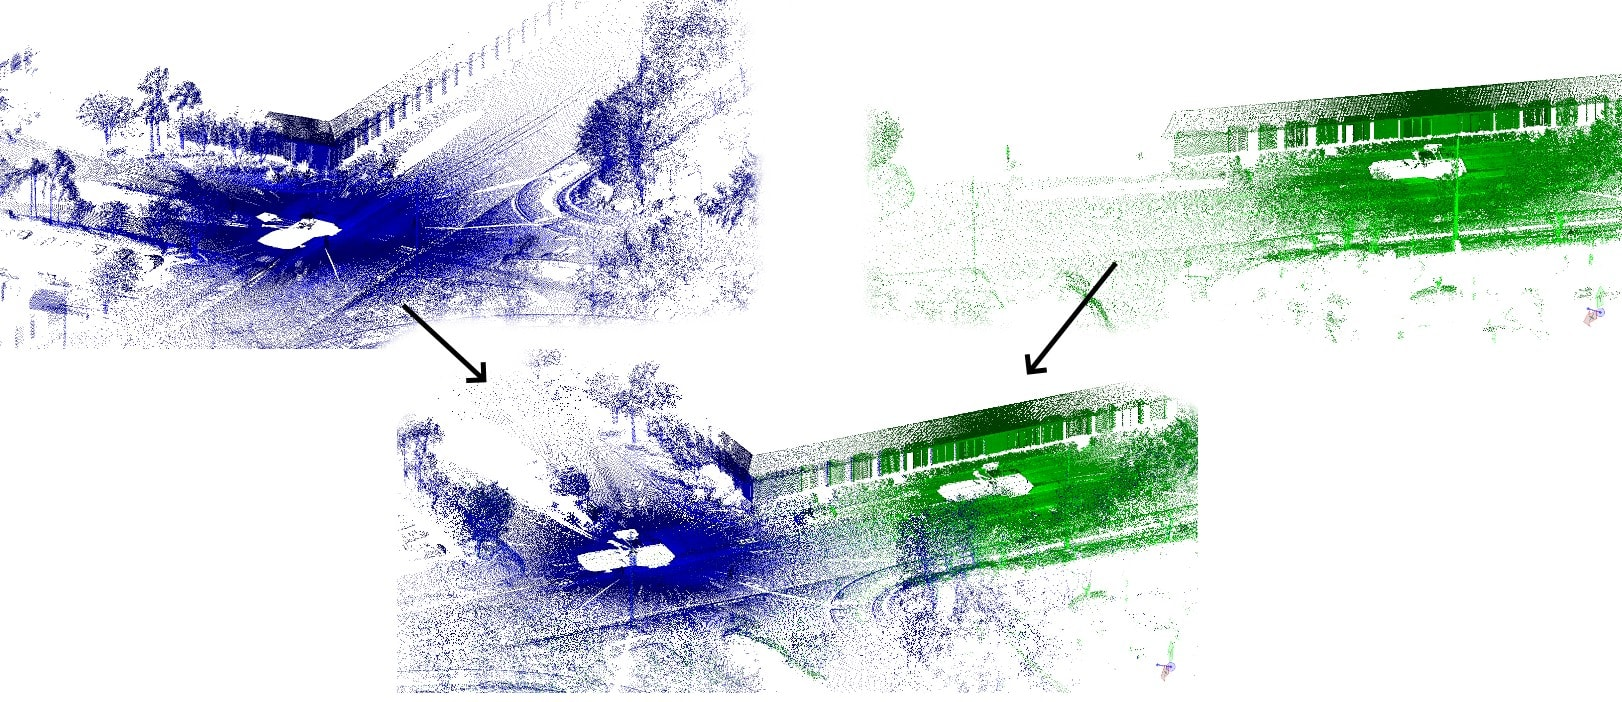
\includegraphics[width=0.7\textwidth]{registration.png}
    \caption{An example of point cloud registration}
    \label{fig:registraion}
\end{figure}

In this part, you are required to implement iterative closest point (ICP) algorithm to find a rigid transformation such that, given two finite size point clouds $\{P,\, Q\}$, the difference between point cloud Q and the transformed point cloud P is minimized. The ICP algorighm can be roughly breaked down into (a) finding a rigid transformation given two point clouds with \textbf{same number of points} and (b) Fixing point cloud Q and iteratively choosing a subset of point cloud P to compute rigid transformation untill convergence.

\begin{algorithm}[h]
\caption{ICP algorithm}\label{alg:icp}
\begin{algorithmic}
\Require source point cloud $p=\{p_i\}^{n_p}$, target point cloud $q=\{q_i\}^{n_q}$, threshold $\epsilon$;
\Ensure A rigid transformation: rotation $R$ and translation $t$;
\State $\bar p \leftarrow \textbf{MEAN}(P), \quad \bar q \leftarrow \textbf{MEAN}(Q)$;
\State $\hat{p_i} = p_i - \bar{p}, \quad \hat{q_i} = q_i - \bar{q}$;
\State $H = \sum_{i=1}^{n_p}{\hat{p_i}\hat{q_i}^T}$

\While{True};
\State $\hat{q}^{'} = \hat{q}.nearestNeighbor(\hat{p})$ \Comment{To find a match and align the pcd size.}
\State $H = \sum_{i=1}^{n_p}{\hat{p_i}\hat{q_i}^T}$
\State $USV^T = SingularValueDecomposition(H)$
\State $ R^* = VU^T$
\State $ t^* = \hat{q}^{'}-R^*\hat{p}$
\State $\hat{p} = R^*\cdot \hat{p} + t^*$
\If{Change of $R$ and $t$ is smaller than threshold $\epsilon$}
break;
\ElsIf{The loss $\sum_{i=1}^{n_p}||(R\cdot p_i+t)-q_i||^2$ is smaller than threshold $\epsilon$}
break;
\ElsIf{Iteraction times exceed the threshold}
break;
\Endif
\Endwhile
\end{algorithmic}
\end{algorithm}
You are required to implement the ICP algorithm from scratch, and third-party libraries can only be used for mathematical computation and visualization. You should visualize at least three pairs of point clouds in your report, and the source and target point cloud should have different colors, as in Figure \ref{fig:registraion}.

\emph{Hint: KD tree is very useful to speed up the algorithm, try it out! (Scipy.spatial.KDTree is a good choice.) If you think the number of points in the point cloud is still too large, you may consider to use some downsample methods like farthest point sampling.}
% ~\\
% ~\\
% ~\\
% ~\\

% \newpage

\section{[20 points] ICP with RANSAC} 
ICP algorithm does not take noisy points into consideraction, and RANSAC is known to be effective in relieving this problem. Please use the RANSAC to reimplement the ICP. More precisely, you should use RANSAC to calculate the rigid transformation in each iteraction of ICP algorithm.

Similarly, third-party libraries can only be used for mathematical computation and visualization. You should visualize at least three pairs of point clouds in your report.


\end{document}
